

To see the full power of the Geometron idea of geometric programming, we must explore how we build custom graphical languages.  Language customization happens by editing the contents of the Geometron Hypercube, the geometric structure described in the Symbols chapter which defines the meanings of geometric actions carried out by the Geometron Virtual Machine.  Each action also has a symbol.  So to create a new graphical language, we decide what graphical elements we want to create, build those, and then also build symbols for each one which fit the format of fitting inside a square with a left to right progression so that they can be part of the glyph spelling we use when creating and editing glyphs.

This chapter is more technical than most people will need or want, and is here for completeness so that the system is fully documented.  Primarily it is a gallery of pictorial examples, and the reader is encouraged on a first reading to skip the text and look at the pictures before moving on to the next section.  This is partly intended as a stub of sorts, a documentation of software which people can re-write to be easier to use as the system evolves.

In principle, there are hundreds of addresses in the Geoemtron Hypercube which we can edit to create custom languages.  These are divided up by function and will be dealt with in different sections of this book.  In practice when we use the basic symbol editor for making 2d web graphics, by far the most commonly used is the Shape Stack.  This is a selection of addresses which are reserved for building languages which have up to 16 shapes, with a matching set of 16 symbols.  The important thing about the Shape Stack is that it gets saved inside each .svg file when they are created in a human readable format which can be extracted back out of the file either automatically or manually.  This is how it is possible to click on a .svg file in the Symbol Feed and have the correct symbol load up and be edited, even when symbols have vastly different specific graphical languages they use.   Engaging the 16 elements of the Shape Stack is done in the default keyboard configuration with capital letters in the second two rows on the keyboard from left to right, or Q, W, E, R, T, Y, U, I, A, S, D, F, G, H, J, K.   

To edit the Shape Stack, we use the shape stack editor which is at shapestack.html.  This is linked via an icon with a 4x4 grid on it.  The shape stack editor uses only the keyboard, and does not have a touch screen interface at the moment.  To edit a shape, you use the customized Geometron keyboard just as you would for creating and editing glyphs in the main symbol editor.  To move to the next and previous shapes, use the up and down arrows.  Try stepping through up and down and get a feel for that.  Also, don't forget that you can use the pan and zoom actions to change your view to zoom in on details you are editing, and that these actions are located at the lowercase ``l'', the semicolon, and n, m and comma and period. 

After you create a new shape, you can change the symbol which represents that shape by clicking on the hypercube icon to go to the shape symbol editor at shapestacksymbols.html.  This is basically the same editor, but pointed at the addresses corresponding to the symbols of the actions you edited in the main editor.  We always want to edit the symbol for a given action so that at the end the cursor is one unit to the right, a square has been drawn, and the state of the GVM is set back to 90 degree angles and factor of 2 scaling.  

The shape stack editor also allows us to trace over images, and you can click on the images in a window which lists the images in the image feeds to select an image, then use the slider bars for scale and rotation to set the image where you need it to in order to trace it.  

As with all elements of the Geometron system, the most important thing we can do with a shape stack is to share it from person to person across the world.  And as always, this information needs to be human readable text in the smallest possible format so that we can copy it to a clipboard and paste it in text messages, emails, directly from browser window to browser window or into pastebins which we can share.  The format for a shape stack is an array of quoted text inside square brackets, separated by commas each of which has an address followed by a colon and then a sequence of addresses which represent the glyph stored at that address.  Once one gains familiarity with the address system of the Geometron Hypercube it is possible to read this code and manipulate it by hand.  However, for people who don't want to dive deeply into any of this, or even to learn how to edit it or interact with it at all, the important thing to know is just that you can use the export and import buttons to exchange shape stacks between one Geometron server and another.  

Also, if you want to see the shape stack used in the creation of a Geometron symbol in .svg format, you can open that symbol in a web browser and use the ``view source'' feature which exists in all browsers. Inside the source code for the .svg you will see a little bit of JSON code at the top inside an XML comment, as well as commented out XML tags which mark where the json is.  This JSON can then be manually copy and pasted into the JSON importer of the whole symbol system or just the shape stack can be removed and used.

If we want to edit and share Hypercubes, we use the Hypercube Editor, also linked from the main symbol app at symbol.html.  This is at hypercube.html on every Geometron server.  In this editor we can edit all parts of the hypercube which contain Geometron glyphs in the byte code format which is sequences of base 8 addresses.  These include all the symbol glyphs, as well as the 8x8 tablets stored in the address ranges starting with 2, 5, and 6.  Once again, we can export and import using buttons and a text area as in all parts of the system.  The actual file being edited with the Hypercube editor is stored at data/hypercube.txt, and you can always look at that in raw plain text and copy it from there as well.  Again, this editor is a sort of stub, and as our swarm grows, more and more people will create their own editors for the Hypercube and various parts of it, as the logic is very simple and it is not hard to make a much better editor than the one presented here. Also, in future editors, the fully three and four dimensional structure can be brought out, using the three dimensional web graphics described in a later chapter.  

The font editor works the same way as the Hypercube editor, with the same basic edit functions but for the range of the Hypercube which holds the font: from 01040 through 01176.  Again, this is designed to be shared, with text based import and export of the human readable text which holds the byte code. The two most important fonts we use are the Robot Font which has pixels which are drawn by the various robots described later, and the Laser Font which has cutouts which when used with a laser cutter can make stencils for spray painting text onto physical objects.  This is part of how we jump the gap from the digital to the physical: text describes a font, text describes a glyph, then that exports to a vector file, and that loads into a laser cutter which makes a stencil which makes a physical link in a physical space which points to a domain which points to the physical location of a server which contains all the information required to replicate that entire system.

The rest of this chapter is simply a gallery of examples of using the shape stack and fonts to make and use different graphical languages to show the potential of Geometron.  Also blank pages and margins can be used to add hand drawn graphics documenting graphical languages for custom illuminated manuscripts to exchange for barter via the Street Network.


\begin{figure}
	\centering
	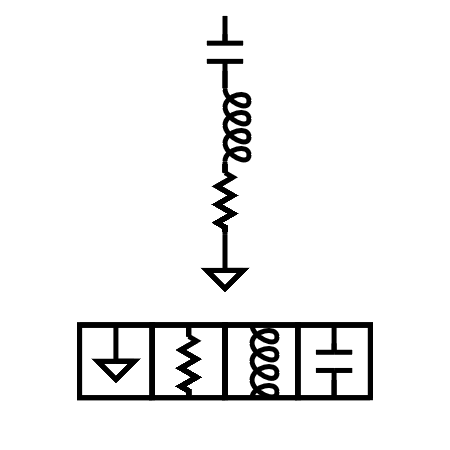
\includegraphics[width=3in]{figures/shapes/rlc.png}
	\caption[RLC]
	{RLC circuit.  Circuit diagrams are a great example of how powerful it is to create a custom graphical language.  Once the schematic symbols for the components are programmed into the Shape Stack and mapped to keys on the keyboard, it is possible to create any circuit diagram with just a few keystrokes.  This simplicity of construction also makes it possible to use any other software tool to generate schematic diagrams automatically.  The symbol glyphs shown spell out the symbol, showing the extreme simplicity of construction once shapes are in place.}
\end{figure}

\begin{figure}
	\centering
	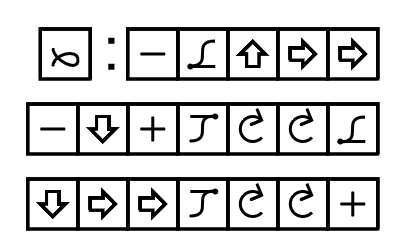
\includegraphics[width=3in]{figures/shapes/inductorloop.png}
	\caption[inductorloop]
	{Construction of a single loop of an inductor.  Once this loop has been created, it can be used to make inductors of any length as well as transformers and any other schematic symbol of something with inductive elements. This shows the power of building up symbols as fractals. Note the geometric precision and simplicity which are not present in the commercial vector graphics packages.}
\end{figure}

\begin{figure}
	\centering
	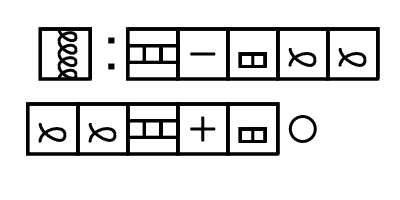
\includegraphics[width=3in]{figures/shapes/inductor.png}
	\caption[inductor]
	{With the loop in place, just a few keystrokes makes a full inductor.}
\end{figure}


\begin{figure}
	\centering
	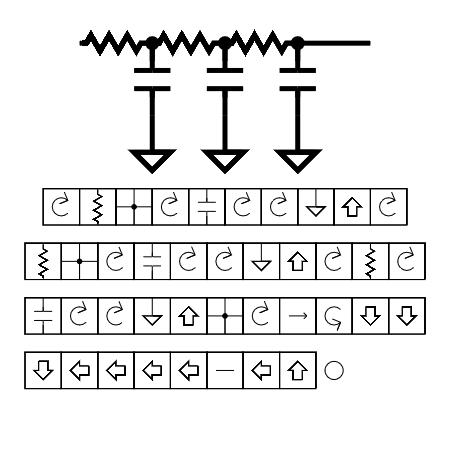
\includegraphics[width=3in]{figures/shapes/rcline.png}
	\caption[RCline]
	{RC line circuit. Another demonstration of the power of Geometron for circuit building.}
\end{figure}

\begin{figure}
	\centering
	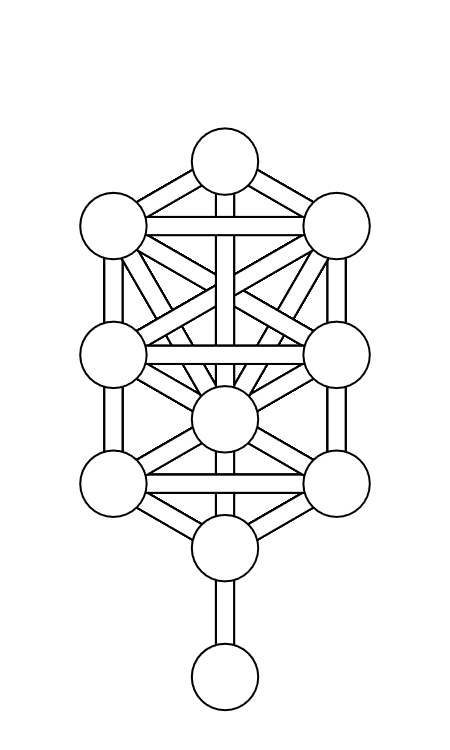
\includegraphics[width=3in]{figures/shapes/treeoflife.png}
	\caption[treeoflife]
	{The Tree of Life from Jewish mysticism.  This symbol also is used in various occult systems.  There is quite a bit of geometry hiding in here, and you can see numerous published examples which get that geometry wrong, breaking the six-fold symmetry of the hexagon.  With Geometron we can build a language for moving around on a hexagon and creating all the various bridges between nodes.}
\end{figure}

\begin{figure}
	\centering
	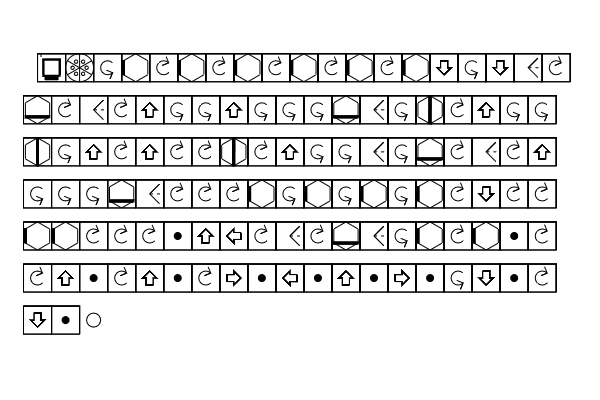
\includegraphics[width=4in]{figures/shapes/treeoflifespelling.png}
	\caption[treeoflifespelling]
	{Symbol glyph spelling of Tree of Life. What makes things like this easy to make is building up building blocks like the cross pieces of all different scales, and the use of universal symmetries and scales(6 fold, 12 fold, and the square root of 3 and 2).}
\end{figure}

\begin{figure}
	\centering
	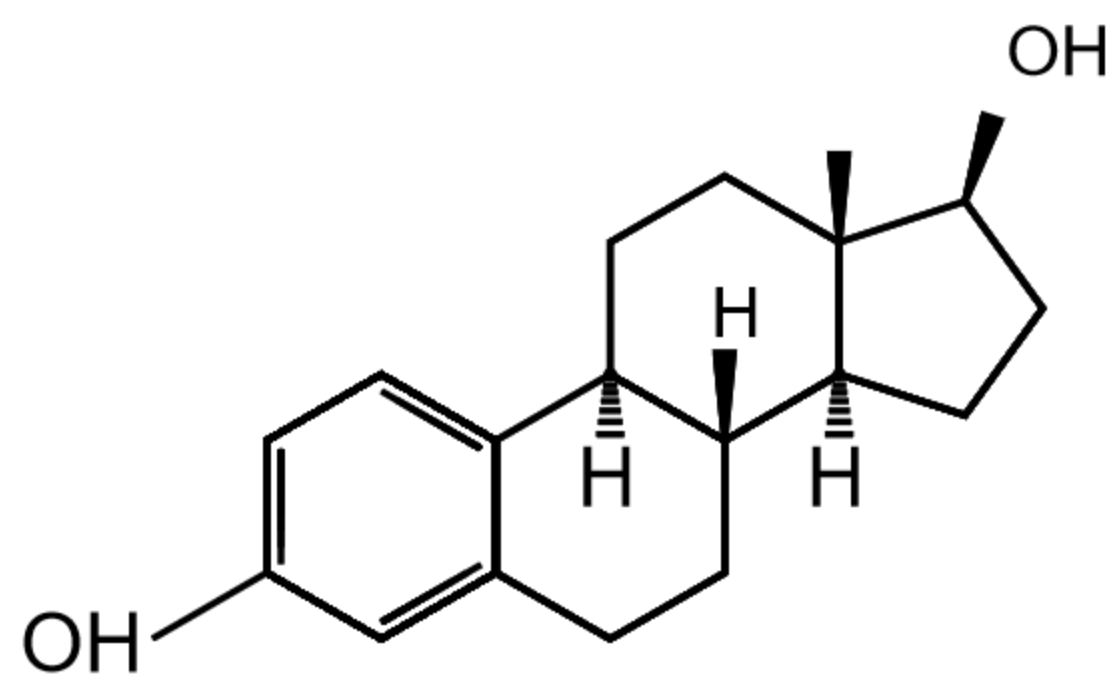
\includegraphics[width=3in]{figures/shapes/estrogendiagram.png}
	\caption[estrogendiagram]
	{Molecular symbol for the steroid hormone estrogen.  Note the characteristic hexagon-pentagon combination which is repeated throughout self-replicating chemical systems(life) as well as throughout the Geometron system/language.}
\end{figure}

\begin{figure}
	\centering
	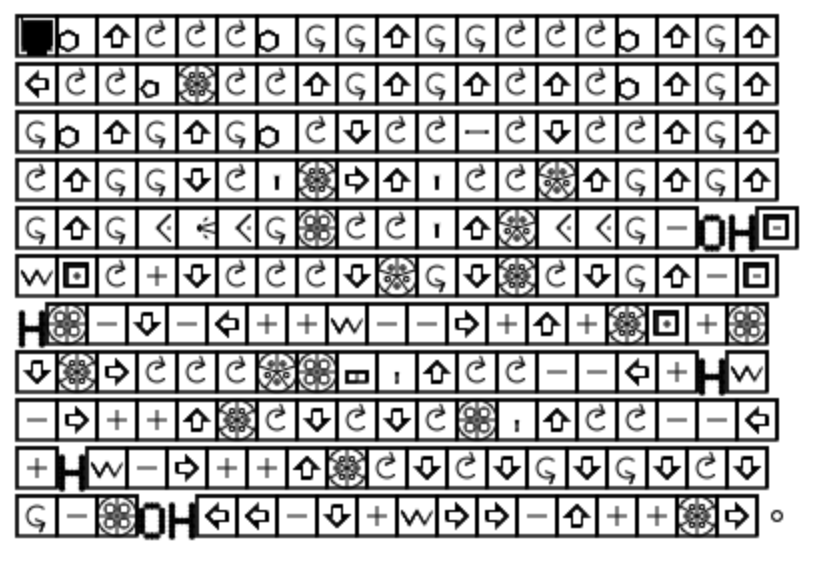
\includegraphics[width=3in]{figures/shapes/estrogenspelling.png}
	\caption[estrogenspelling]
	{Symbolic spelling of the chemical symbol in the previous figure.  This spelling is only possible because of constructing a symbolic language specific to drawing organic chemistry symbols.}
\end{figure}

\begin{figure}
	\centering
	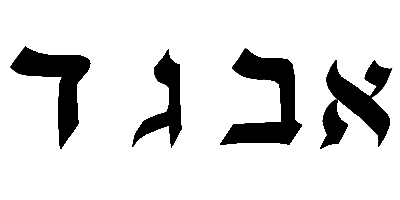
\includegraphics[width=3in]{figures/shapes/hebrew.png}
	\caption[hebrew]
	{Some letters from a Hebrew font. Typesetting a language which goes from right to left is a powerful demonstration of the way Geometron works.  Each letter is a sequence of geometric actions, just as it is when a human uses a pen to create it.  This means that if the actions end with the cursor to the left or bottom or diagonally that is where the next letter will be.  There is no need to mode switch based on direction, the direction is built into each individual character.}
\end{figure}


\begin{figure}
	\centering
	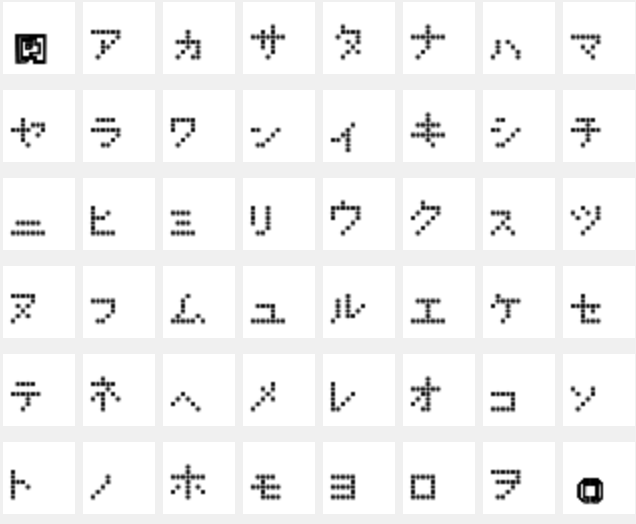
\includegraphics[width=3in]{figures/shapes/katakana.png}
	\caption[katakana]
	{A katakana font using pixels.  Again, we can create this with a sense of direction built in, which for Japanese has a few choices. We make this vertical so that it can be used to make Matrix rain, which is katakana in mirror writing. The font is made as regular characters, and then by simply changing the value in the hypercube of movement from left to right and from right to left from pixel to pixel, the katakana can be made mirrored or not without affecting the actual font elements.}
\end{figure}

\begin{figure}
	\centering
	
\includegraphics[width=3in]{figures/shapes/blank.png}
\end{figure}
\begin{figure}
	\centering
	
\includegraphics[width=3in]{figures/shapes/blank.png}
\end{figure}
\begin{figure}
	\centering
	
\includegraphics[width=3in]{figures/shapes/blank.png}
\end{figure}
\begin{figure}
	\centering
	
\includegraphics[width=3in]{figures/shapes/blank.png}
\end{figure}
\begin{figure}
	\centering
	
\includegraphics[width=3in]{figures/shapes/blank.png}
\end{figure}
